%! TEX root = **/000-main.tex
% vim: spell spelllang=en:

\section{Visão Geral}%
    \subsection{Tema/Contexto/gênero}%
    \label{sec:contexto}
    A tematica principal do jogo será a de frutos do mar, sendo usados tanto elementos biologia/vida marinha quanto de seus usos culinarios.
    Para trazer essa ideia a vida sera usado o gênero de platformer com elementos de ação, sendo um tradicional "corre e atira".\\

    \subsection{Mecânicas Central}%
    \label{sec:mecanica}
    Como mencionado em \Cref{sec:contexto} o jogo será um "corre e atira" logo as principais mecânicas serão as de movimentação e combate.\\

        \subsubsection{Movimentação}\label{sec:mecanica:movimentação}

        \begin{itemize}
        \item andar para a esquerda
        \item andar para a direita
        \item saltar
        \item mecânica de dash
        \end{itemize}

        \subsubsection{Combate}\label{sec:mecanica:combate}
        Já no combate, haverá 2 ataques disponiveis para o jogador:

        \begin{itemize}
          \item Um ataque a curta distância usando a pinça, o ataque percorrera uma curta faixa logo a frente do protagonista, dando dano em tudo naquela area.
          \item Um ataque a distância, sendo um disparo de agua emitido da pinça do personagem, percorre uma distância muito maior que o ataque melee, porém causando menos dano, e que depende de munição (agua) para ser ultilizado.
        \end{itemize}

    \subsection{Plataformas Alvo}%
    Inicialmente PC:
        \begin{itemize}
            \item Windowns
            \item Linux
        \end{itemize}
    Porém com possivel expanção para consoles em caso de sucesso.
    \subsection{Público Alvo}%
        Publico jovem, gen z, que gostam do tipo de humor nonsense, afinal o protagonista é um camarão solitário em busca de amor, mas que não abrem mão da experiencia de jogar um bom platformer.

    \subsection{Escopo do Projeto}%
    \subsubsection{Tempo de desenvolvimento}
        De 3 a 4 meses.
    \subsubsection{Equipe}
        \begin{itemize}
            \item Silmar Pereira da Silva Junior: Programação, Design, DevOps;
            \item João Paulo Garcia Martinelli de Oliveira: programação e arquitetura dos leveis;
            \item Lucas Gabriel Mendes Miranda: design;
            \item Flavio Ippolito Vasini Design;
            \item Leonardo Vinícius de Almeida: programador;
        \end{itemize}

    \subsection{Influências}%
        \subsubsection{Megaman:}
        \label{sec:influencias:megaman}
            \begin{figure}[H]
                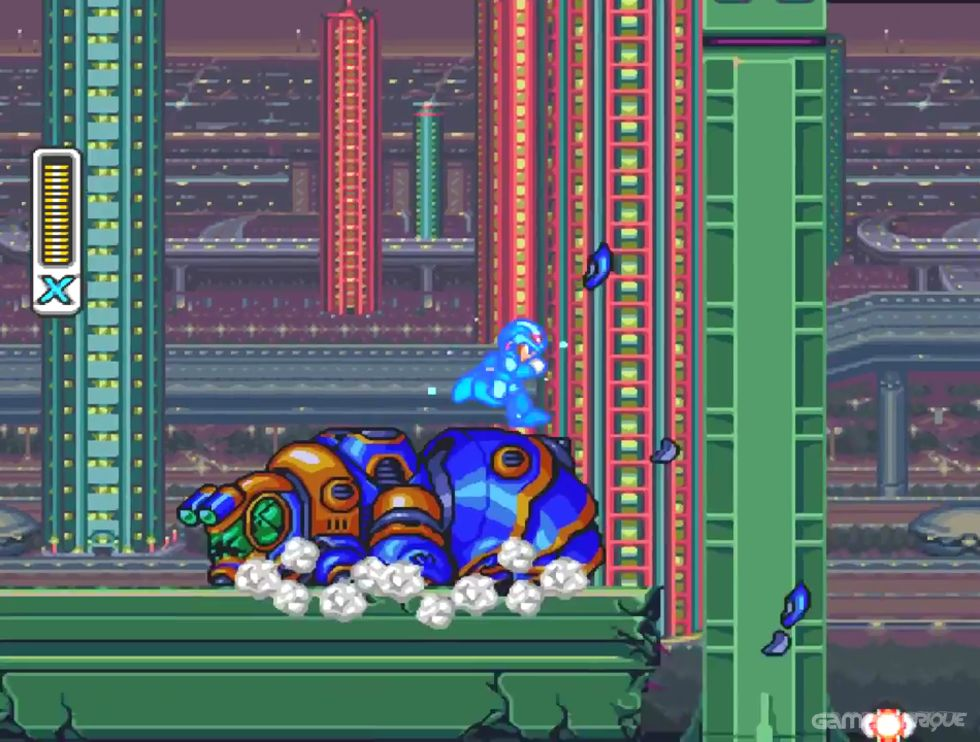
\includegraphics[width=8cm]{Megaman}
            \centering
            \end{figure}

        Megaman é a principal referência quanto ao gameplay, bastante da mecânica é inspirada no jogo, como mencionado na \Cref{sec:mecanica}, correr, pular e atirar são as principais atividades desenpenhadas por X (protagonista do Megaman X) e pelo camarão. Ademais, em subsequentes jogos da franquia, houve a adição de mais um personagem jogável, o Zero, que usa sua espada para causar ataques de curta distância, dos quais o golpe melee do protagonista é baseado.\\
        Além das mecânicas de movimentação e combate, outro elemento que Megaman servirá de inspiração será no level design, com fases bem projetadas para oferecer desafios ao jogador e um boss no final.\\

        \subsubsection{Cuphead:}
            \begin{figure}[H]
                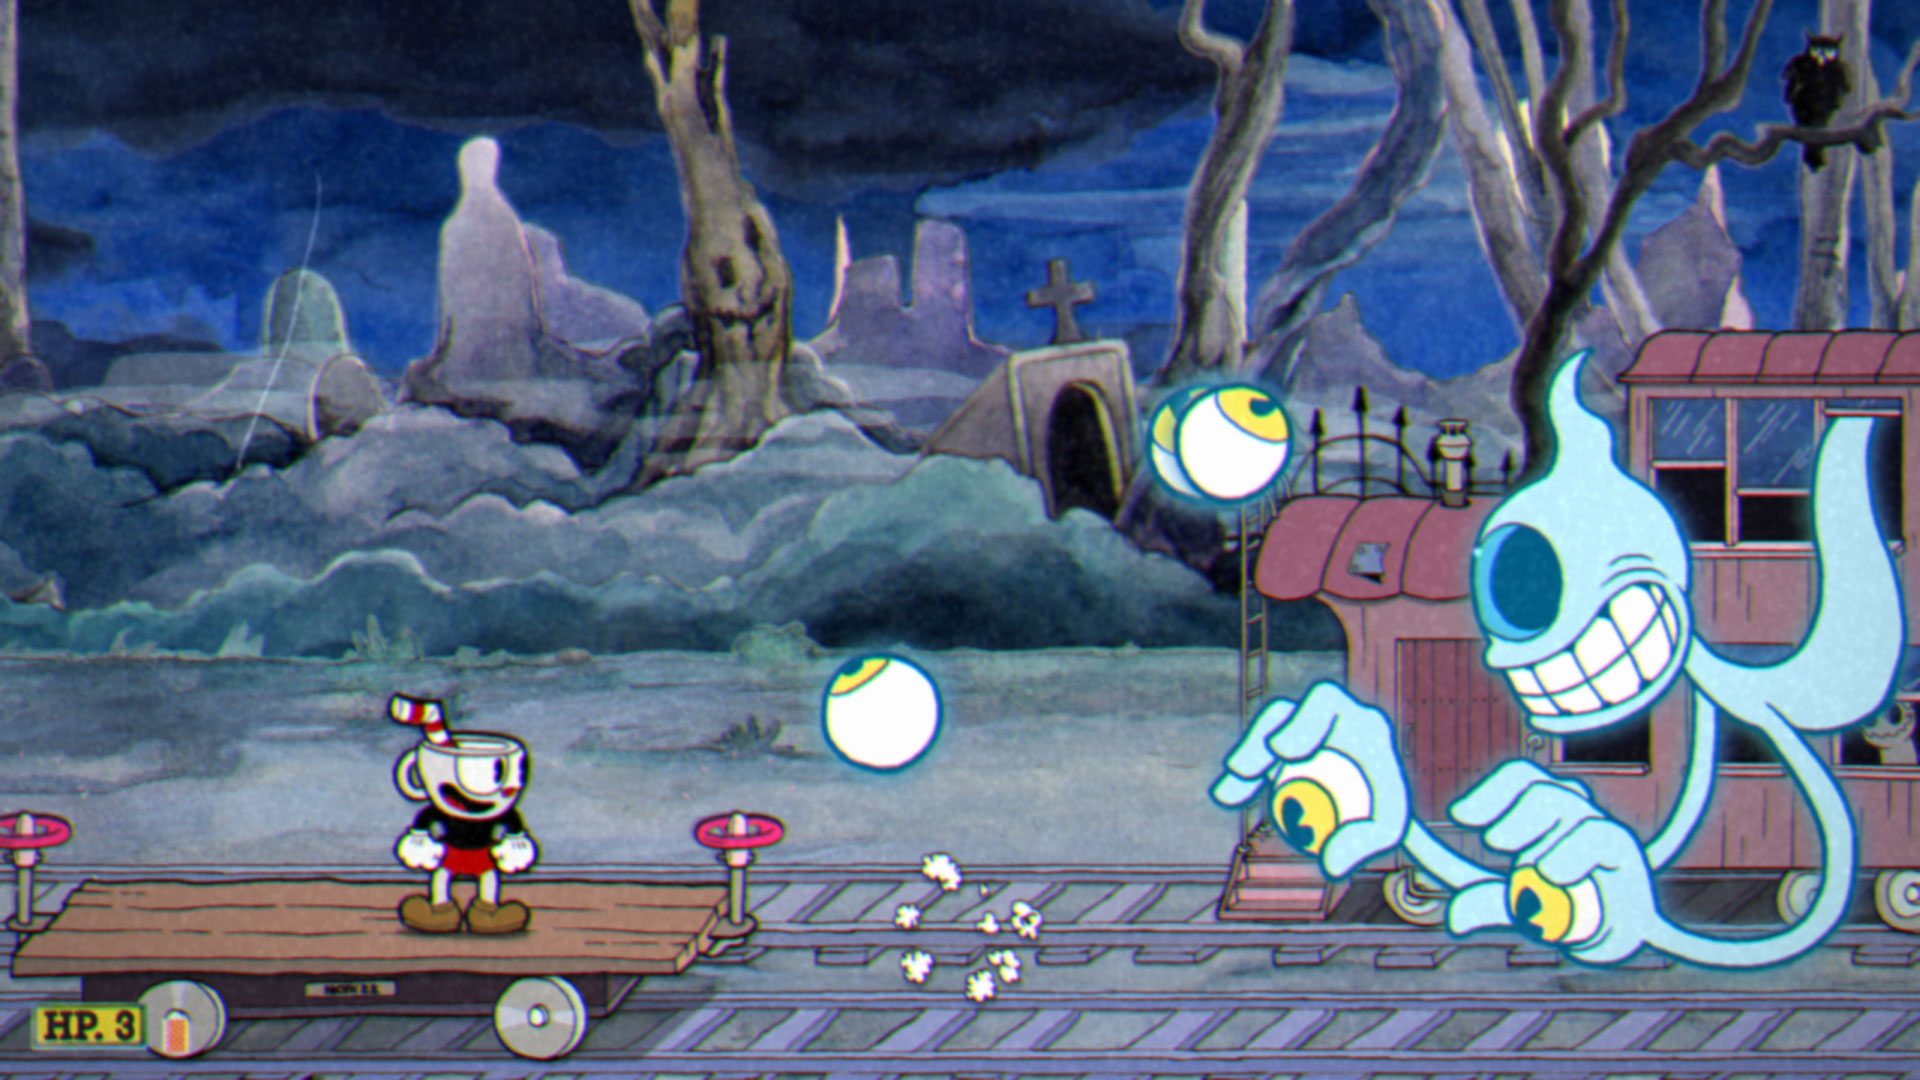
\includegraphics[width=10cm]{Cuphead}
            \centering
            \end{figure}

            Cuphead, será a inspiração quanto ao design de personagens, cenários, inimigos e tudo relacionado ao artistico do projeto, sendo bem colorido e cartunesco.\\
            Também vale resaltar que varias das mecânicas mencionadas em \Cref{sec:influencias:megaman} são compartilhadas com Cuphead e também serão consideradas como formas de inspiração, apesar das influências usadas de Cuphead serem mais voltadas ao artístico e nem tanto ao gameplay.\\

        \subsubsection{Biologia:}
            \begin{figure}[H]
                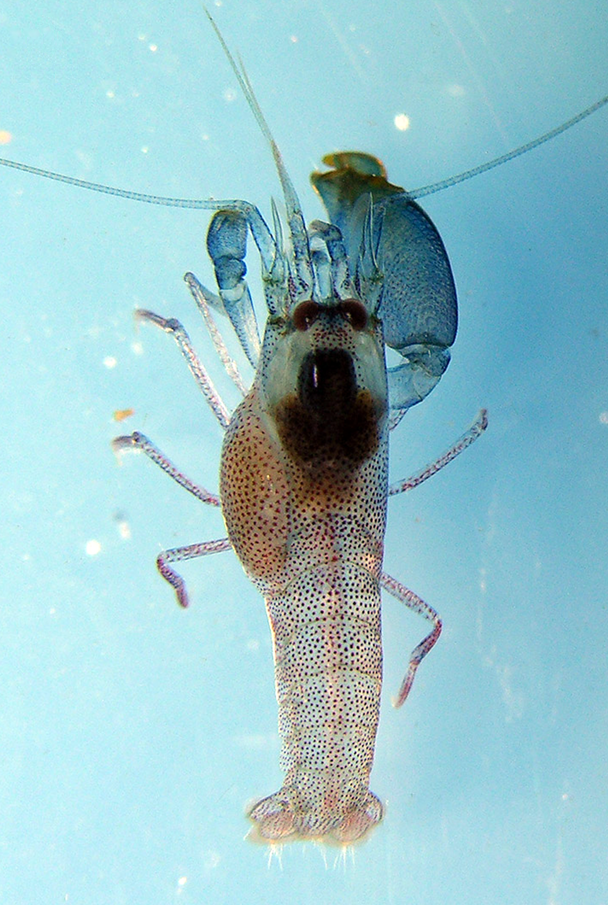
\includegraphics[width=5cm]{PistolShrimp}
            \centering
            \end{figure}

            A especie de camarão \textit{Synalpheus fritzmuelleri} mais conhecida como camarão-pistola é a grande inspiração para o protagonista do jogo, essa especie possui uma pinça direita peculiar, que é capaz de ao fechar e precionar a agua dentro dela produz uma onda de choque que se move pela agua tão forte que é capaz de nocautear suas presas.
 
        \subsubsection{CupNoodles de frutos do mar:}
            \begin{figure}[H]
                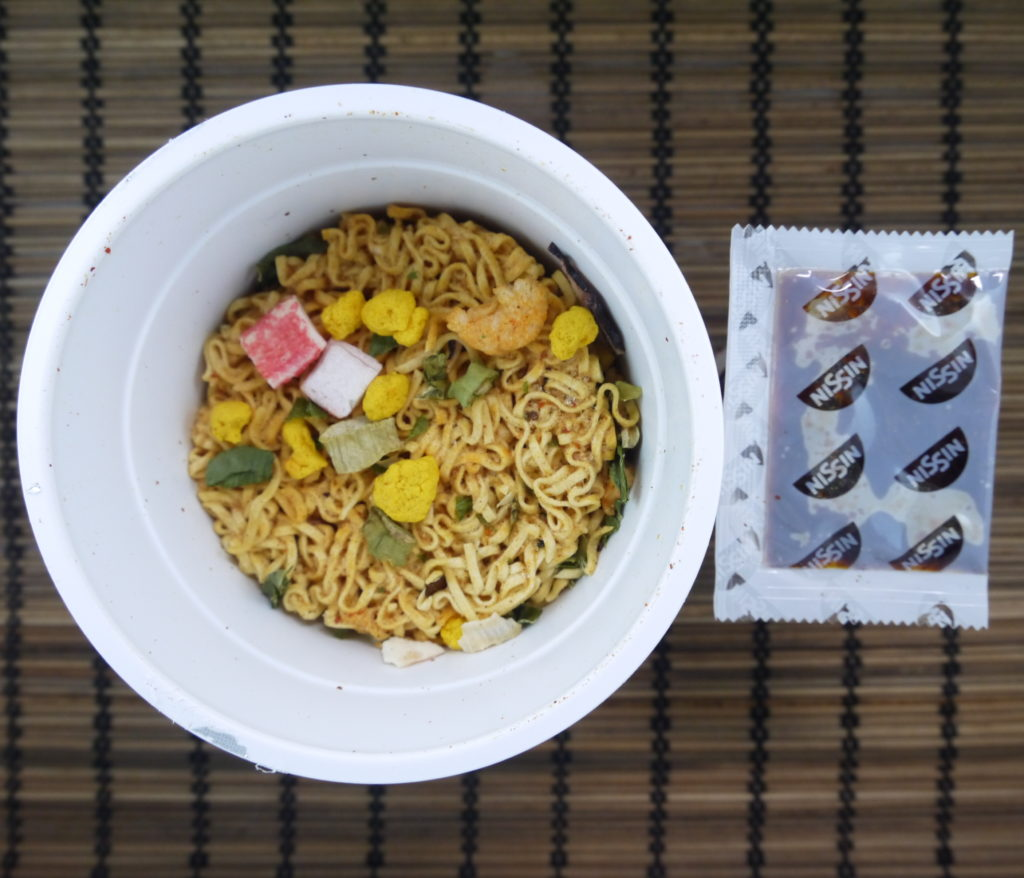
\includegraphics[width=10cm]{CupNoodles}
            \centering
            \end{figure}
            
            Todo CupNoodles tem acompanhamentos que vem junto do macarrão e no de frutos do mar não é diferente, mas já tentou achar um camarão nele, garantimos que há no maximo 1 por pacote, ele está lá, sozinho, apenas esperando que se ponha agua quente, espere 3 minutinhos e acabe com sua solidão.

    \subsection{Descrição do projeto}%
Em um cup noodles de frutos do mar, o unico camarão desidratado do pacote, solitário e na escuridão, tenta escapar de sua prisão, para voltar ao mar em busca de seu amor.\\
Embarque nessa jornada cheia de perigos e plataformas, usando sua poderosa pinça para esmagar inimigos que ficarem entre seu você e o amor verdadeiro, e se não ousarem chegar basta bater suas pinças para criar um pulso de agua capaz de destruir qualquer um.\\
Nada pode parar um camarão determinado\\

    \subsection{Controles}%
    \begin{figure}[H]
        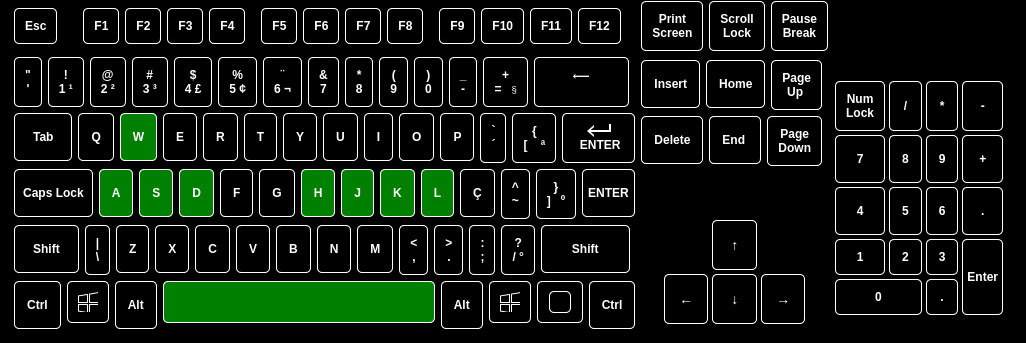
\includegraphics[width=10cm]{keys}
    \centering
    \end{figure}

    Para o gameplay serão usados as teclas com a seguinte disposição:
    \begin{itemize}
        \item Movimentação
        \begin{itemize}
            \item A  - anda para a esquerda
            \item AA - dash para a esquerda
            \item D  - anda para a direita
            \item DD - Dash para a direita
            \item S  - aguaixar
            \item W  - Olhar para cima
            \item ESPAÇO - pula
        \end{itemize}
 
        \item Combate
        \begin{itemize}
            \item J - ataque melee
            \item K - ataque ranged
        \end{itemize}

        \item Misc
        \begin{itemize}
            \item H - interage com o cenario e items
        \end{itemize}

    \end{itemize}
    
\section{História/Lore}%
    \begin{figure}[H]
        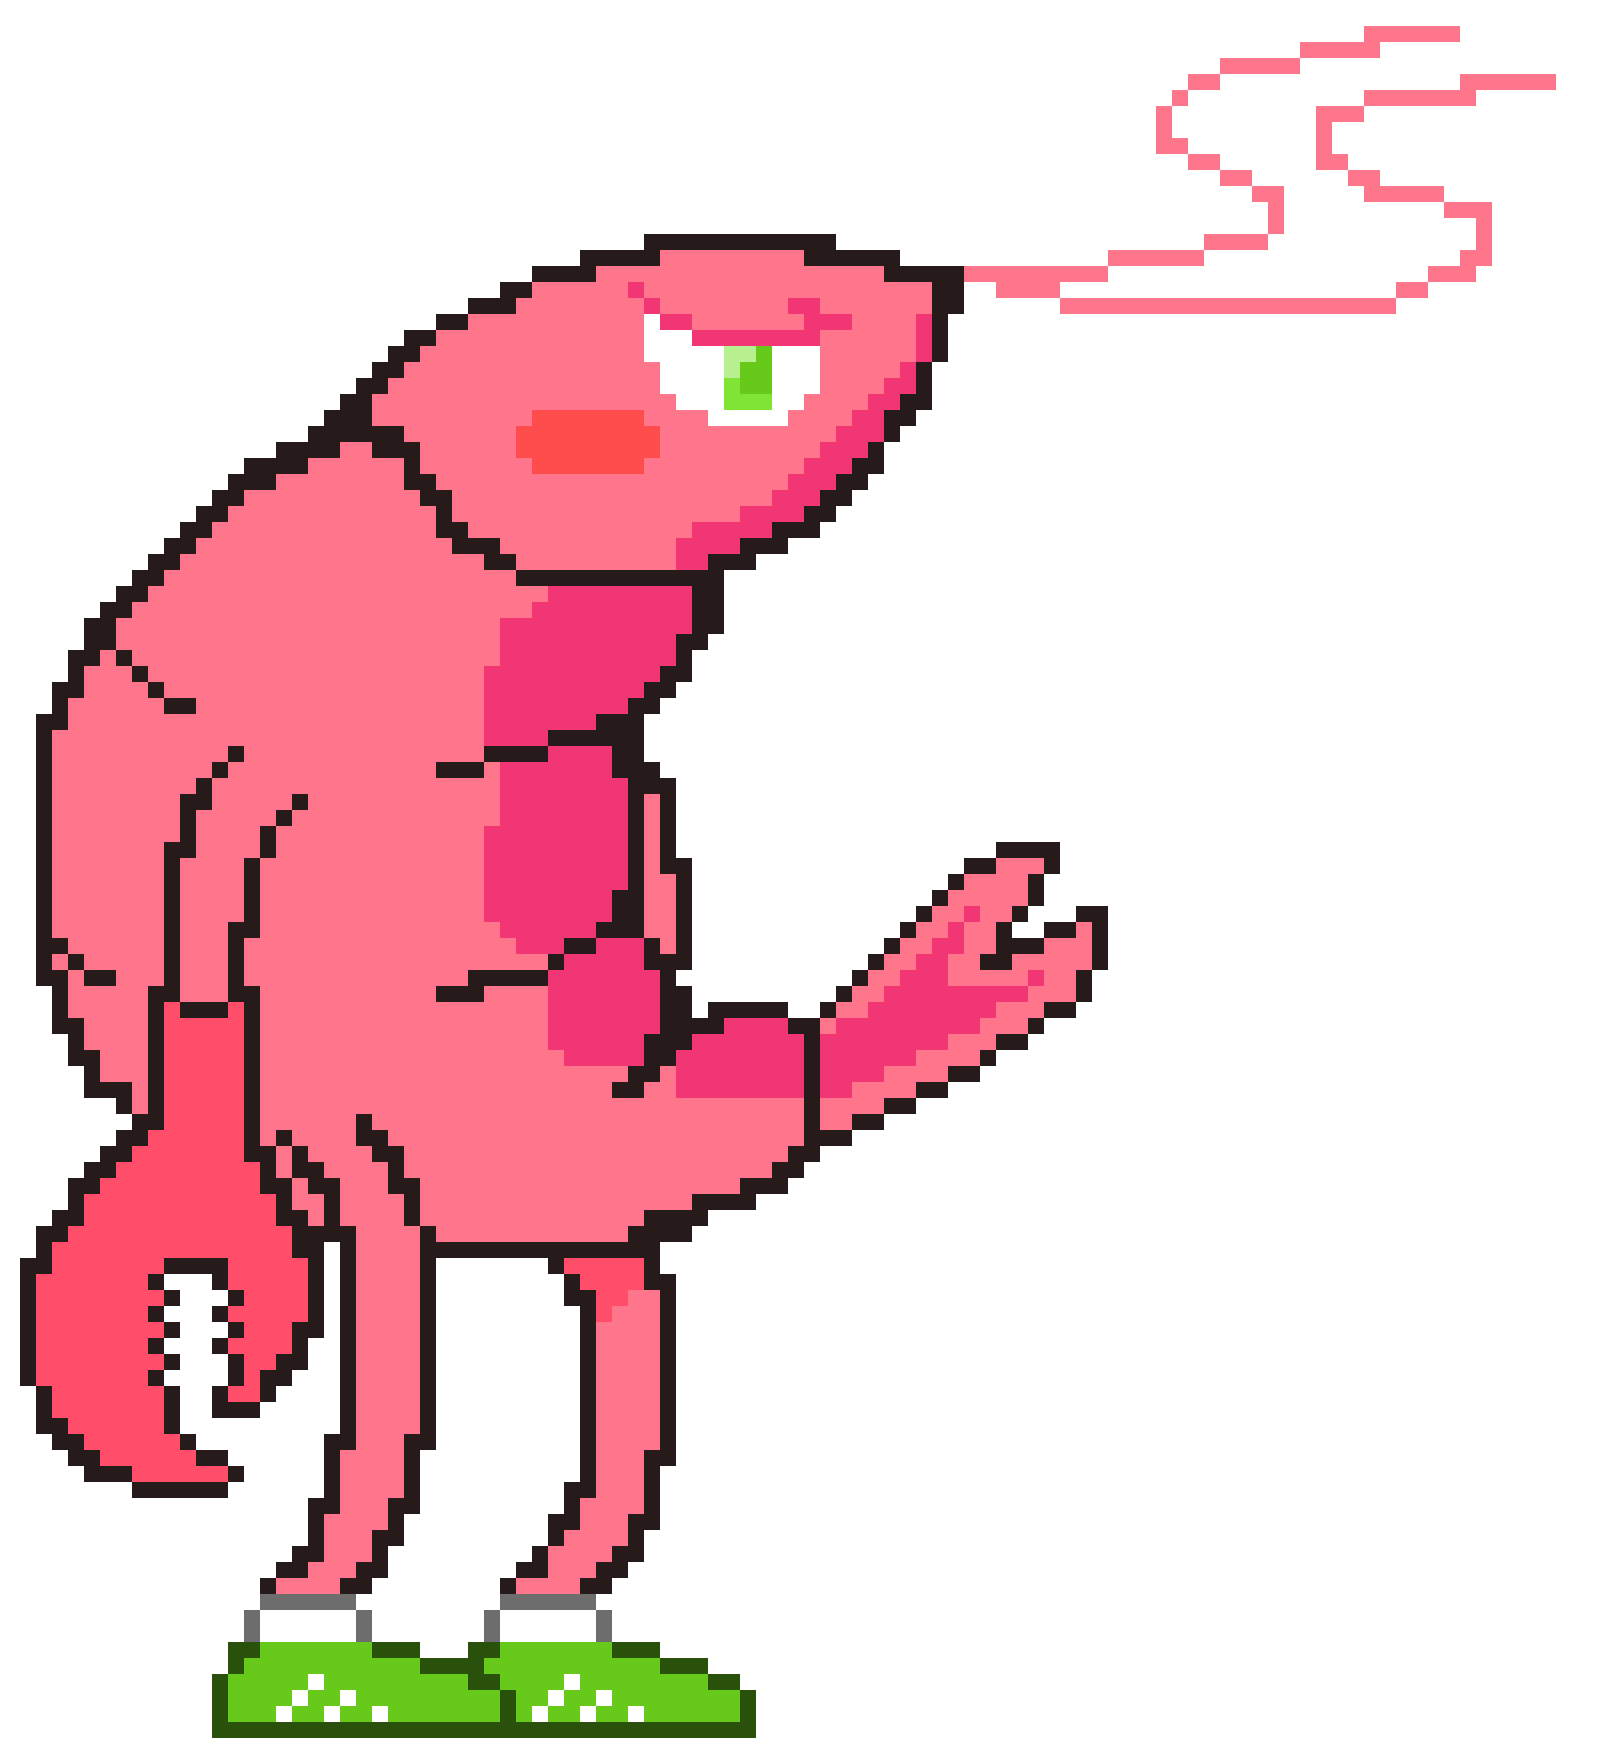
\includegraphics[width=5cm]{shrimp1--prot}
    \centering
    \end{figure}


    A lore do jogo consiste na história de um camarão, que após ser capiturado, desidratado e parar em um pode de capNoodles (para evitar problemas com direitos autorais) volta a vida e ao se sentir extremamente só, decide tentar escapar de sua prisão e tentar regressar ao mar para encontrar seu amor. A partir desse ponto ele viajará por diversos ambientes até chegar em seu objetivos, se encontrando com diversos conhecidos e não conhecidos, que revelarão dicas sobre ele proprio e os desáfios que irá encontrar, além de vários possíveis plot twists.
